\documentclass[11pt,a4paper]{article}

% --- Geometry & Margins ---
\usepackage[margin=20mm]{geometry}

% --- Typography & Font Setup ---
\usepackage{times}              % Times New Roman equivalent for body text
\usepackage{helvet}             % Arial/Helvetica equivalent for headings
\usepackage[T1]{fontenc}
\usepackage[utf8]{inputenc}
\usepackage{microtype}
\usepackage{setspace}
\setstretch{1.15}               % 1.15 line spacing

% --- Paragraph Formatting ---
\setlength{\parindent}{0pt}
\setlength{\parskip}{6pt}       % 6 pt after body paragraphs

% --- Packages for Tables & Layout ---
\usepackage{tabularx}
\usepackage{booktabs}
\usepackage{array}
\usepackage{enumitem}
\usepackage{titlesec}
\usepackage{tikz}
\usetikzlibrary{shapes.geometric, arrows.meta, positioning}
\usepackage{amssymb}            % For checklist boxes (\square)
\usepackage[colorlinks=true, linkcolor=blue, urlcolor=blue, citecolor=blue]{hyperref}

% --- Section Heading Formatting (Arial-like Sans-Serif) ---
\titleformat{\section}
  {\sffamily\large\bfseries}{\thesection.}{0.5em}{}
\titleformat{\subsection}
  {\sffamily\normalsize\bfseries}{\thesubsection}{0.5em}{}
\titleformat{\subsubsection}
  {\sffamily\normalsize\bfseries}{\thesubsubsection}{0.5em}{}

% --- Table Helpers ---
\newcolumntype{L}[1]{>{\raggedright\arraybackslash}p{#1}}
\newcolumntype{Y}{>{\raggedright\arraybackslash}X}
\renewcommand{\arraystretch}{1.2}

\begin{document}

% =========================================================================
% PAGE 1: VISUAL SYNOPSIS & METADATA
% =========================================================================

\begin{center}
    {\sffamily\Large\textbf{Khulna University of Engineering \& Technology}}\\[0.2em]
    {\sffamily\large\textbf{Department of Computer Science and Engineering}}\\[0.2em]
    {\sffamily\normalsize\textbf{CSE 4112: Machine Learning Laboratory}}\\[0.8em]
    {\sffamily\LARGE\textbf{DATASET REPORT}}\\[0.6em]
    {\sffamily\large [Dataset Title: include the words ``data'' or ``dataset'' where appropriate]}
\end{center}

\vspace{0.5em}

\noindent
\begin{tabularx}{\textwidth}{|p{3.2cm}|X|p{3.2cm}|X|}
\hline
\textbf{Group No.} & [\_\_] & \textbf{Dataset Version} & [v1.0 / date] \\
\hline
\textbf{Students} & [Names \& rolls of 6 members] & \textbf{Repository} & [URL/DOI if available] \\
\hline
\end{tabularx}

\vspace{1.5em}

% --- Pipeline Diagrams (TikZ) ---
\noindent
\textbf{(a) Framework illustrating the practical application of the data}

\vspace{0.4em}
\noindent
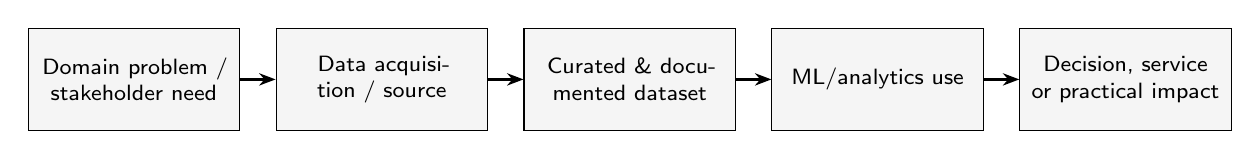
\begin{tikzpicture}[
    node distance=0.45cm,
    block/.style={rectangle, draw, fill=gray!8, text width=2.45cm, minimum height=1.3cm, align=center, font=\footnotesize\sffamily},
    arrow/.style={-{Stealth[scale=0.9]}, thick}
]
    \node[block] (b1) {Domain problem / stakeholder need};
    \node[block, right=of b1] (b2) {Data acquisition / source};
    \node[block, right=of b2] (b3) {Curated \& documented dataset};
    \node[block, right=of b3] (b4) {ML/analytics use};
    \node[block, right=of b4] (b5) {Decision, service or practical impact};

    \draw[arrow] (b1) -- (b2);
    \draw[arrow] (b2) -- (b3);
    \draw[arrow] (b3) -- (b4);
    \draw[arrow] (b4) -- (b5);
\end{tikzpicture}

\vspace{0.3em}
\noindent
{\footnotesize\textbf{Figure 1(a).} Replace the generic boxes with a dataset-specific application framework; identify the intended users and practical outcome.}

\vspace{1.2em}

\noindent
\textbf{(b) Technical pipeline of the ML method using the dataset}

\vspace{0.4em}
\noindent
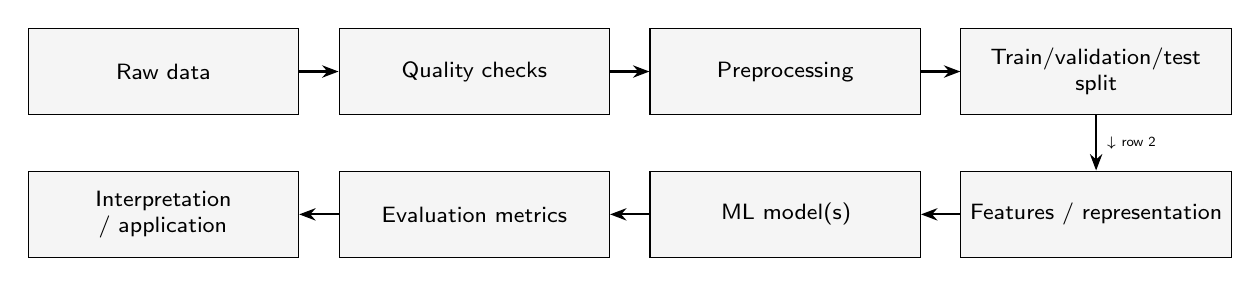
\begin{tikzpicture}[
    node distance=0.7cm and 0.5cm,
    block/.style={rectangle, draw, fill=gray!8, text width=3.2cm, minimum height=1.1cm, align=center, font=\footnotesize\sffamily},
    arrow/.style={-{Stealth[scale=0.9]}, thick}
]
    % Row 1
    \node[block] (p1) {Raw data};
    \node[block, right=of p1] (p2) {Quality checks};
    \node[block, right=of p2] (p3) {Preprocessing};
    \node[block, right=of p3] (p4) {Train/validation/test split};

    % Row 2
    \node[block, below=of p4] (p5) {Features / representation};
    \node[block, left=of p5] (p6) {ML model(s)};
    \node[block, left=of p6] (p7) {Evaluation metrics};
    \node[block, left=of p7] (p8) {Interpretation / application};

    % Connectors
    \draw[arrow] (p1) -- (p2);
    \draw[arrow] (p2) -- (p3);
    \draw[arrow] (p3) -- (p4);
    \draw[arrow] (p4) -- (p5) node[midway, right, font=\tiny\sffamily] {$\downarrow$ row 2};
    \draw[arrow] (p5) -- (p6);
    \draw[arrow] (p6) -- (p7);
    \draw[arrow] (p7) -- (p8);
\end{tikzpicture}

\vspace{0.3em}
\noindent
{\footnotesize\textbf{Figure 1(b).} Replace with the exact technical pipeline to be followed in the course project. Show leakage-safe splitting and dataset transformations clearly.}

\vspace{1.5em}
\hrule
\vspace{0.5em}

\noindent
{\footnotesize\textbf{FIRST-PAGE RULE:} Keep Page 1 as a visual synopsis. Use concise labels; detailed explanations belong in the main report.}

\clearpage

% =========================================================================
% PAGE 2+: REPORT PREPARATION AND SUBMISSION FORMAT
% =========================================================================

\section*{REPORT PREPARATION AND SUBMISSION FORMAT}
This is a course-specific dataset report template. It combines the reporting logic of \textit{Data in Brief} with common data-descriptor elements used by \textit{Scientific Data} and \textit{MDPI Data}, and adds an ML-readiness/baseline section for CSE 4112.

\vspace{0.5em}

\noindent
\begin{tabularx}{\textwidth}{|p{4.0cm}|X|}
\hline
\textbf{Paper \& margins} & A4 (210 $\times$ 297 mm); approximately 20 mm margins. \\
\hline
\textbf{Font} & Times New Roman, 11 pt body; Arial for headings/figures. Keep formatting consistent. \\
\hline
\textbf{Spacing} & 1.15 line spacing; 6 pt after body paragraphs. Single spacing is acceptable in tables/captions. \\
\hline
\textbf{Recommended length} & About 8–12 pages after Page 1, excluding appendices. Quality and completeness are more important than page count. \\
\hline
\textbf{Figures \& tables} & Number consecutively; cite every figure/table in the text; captions must be self-explanatory. \\
\hline
\textbf{References} & Numbered citation style in square brackets. Prefer dataset papers, data-collection sources, instruments/software, and relevant ML references. \\
\hline
\textbf{Submission files} & One report (DOCX/PDF as instructed), dataset/repository link, README, data dictionary, and code/notebook link where applicable. \\
\hline
\end{tabularx}

\vspace{1.5em}

% --- SECTION 1 ---
\section{Dataset Article Information}
\noindent
\begin{tabularx}{\textwidth}{|p{4.2cm}|X|}
\hline
\textbf{Dataset/report title} & [Concise title; clearly indicate the dataset and domain] \\
\hline
\textbf{Group and students} & [Group no.; 6 students with names and rolls] \\
\hline
\textbf{Affiliation} & Department of CSE, KUET, Khulna-9203, Bangladesh \\
\hline
\textbf{Corresponding student} & [Name, roll, institutional email] \\
\hline
\textbf{Keywords} & [4–8 keywords; avoid simply repeating the title] \\
\hline
\textbf{Dataset version} & [e.g., v1.0; release date] \\
\hline
\textbf{Repository / persistent ID} & [Repository name; DOI/URL; “Not yet public” only if instructor permits] \\
\hline
\textbf{License} & [e.g., CC BY 4.0, CC0, or justified restricted-access terms] \\
\hline
\textbf{Related article / source} & [Citation or “None”] \\
\hline
\end{tabularx}

\vspace{1.5em}

% --- SECTION 2 ---
\section{Abstract}
Write 150–300 words. Describe why the dataset was created, how data were collected/compiled, what the dataset contains, its scale/formats, quality-control approach, and how it may be reused. Do not turn the abstract into a results or conclusion section.

[Write the abstract here.]

\vspace{1.5em}

% --- SECTION 3 ---
\section{Dataset Specifications Table}
\noindent
\begin{tabularx}{\textwidth}{|p{4.2cm}|X|}
\hline
\textbf{Item} & \textbf{Required information} \\
\hline
\textbf{Subject / domain} & [Broad area: e.g., agriculture, health, transport, environment, education, cybersecurity] \\
\hline
\textbf{Specific subject area} & [Precise scope of the dataset] \\
\hline
\textbf{Type of data} & [Tabular / image / audio / video / text / time series / sensor / multimodal; raw and/or processed] \\
\hline
\textbf{File formats} & [CSV, XLSX, JSON, JPG, WAV, TXT, etc.; state open/non-proprietary formats where possible] \\
\hline
\textbf{Unit of observation} & [What does one row/image/record/sample represent?] \\
\hline
\textbf{Data collection / source} & [Primary collection, survey, sensor, web/API, public source, secondary compilation, etc.] \\
\hline
\textbf{Instrument / software} & [Device, model, app, script, library, version] \\
\hline
\textbf{Data source location} & [Geographic/source location and collection setting] \\
\hline
\textbf{Collection period} & [Start/end date or relevant time window] \\
\hline
\textbf{Dataset size} & [No. of records/files/classes/features; storage size if relevant] \\
\hline
\textbf{Target / labels} & [Prediction target(s), class labels, annotation scheme, or “Not applicable”] \\
\hline
\textbf{Accessibility} & [Repository, DOI/persistent ID, direct URL, access instructions] \\
\hline
\textbf{License / reuse terms} & [License and any ethical/access constraints] \\
\hline
\end{tabularx}

\vspace{1.5em}

% --- SECTION 4 ---
\section{Value of the Data}
Provide 3–6 concise bullet points. Explain why the data are useful, who can reuse them, what research/engineering questions they can support, and what makes the dataset practically relevant. Avoid unsupported claims of novelty or superiority.
\begin{itemize}[leftmargin=1.5em, itemsep=2pt, topsep=2pt]
    \item [Why is this dataset valuable?]
    \item [Who is likely to reuse it?]
    \item [What ML/data-mining tasks can it support?]
    \item [How can it be extended, combined, benchmarked, or compared with other data?]
\end{itemize}

\vspace{1em}

% --- SECTION 5 ---
\section{Background and Practical Motivation}
Explain the real-world problem and the motivation for creating the dataset. Briefly position it relative to existing datasets or data-collection practices. Refer back to the practical-application framework on Page 1. Recommended: 200–400 words.

[Background, context, gap, stakeholders, and motivation.]

\vspace{1.5em}

% --- SECTION 6 ---
\section{Data Acquisition / Experimental Design, Materials and Methods}
Describe data generation/collection in enough detail that another group could reproduce the process. Distinguish primary data from externally sourced/secondary data.

\subsection{Data source and sampling strategy}
[Population/source frame, sampling method, inclusion/exclusion criteria, sample size rationale where relevant.]

\subsection{Collection setting, period and location}
[Where, when, under what conditions, and by whom the data were collected.]

\subsection{Instruments, hardware, software and versions}
[Device make/model, sensors, apps, scripts, libraries, APIs, questionnaire sources, settings/parameters.]

\subsection{Variables, measurements and metadata}
[What was measured/recorded; units; feature definitions; metadata captured.]

\subsection{Annotation / labeling protocol}
[Who labeled the data; label definitions; instructions; adjudication; inter-rater agreement if applicable.]

\subsection{Provenance, versioning and raw-data preservation}
[How raw data were preserved; naming/version rules; transformation history; source URLs/identifiers for secondary data.]

\vspace{1.5em}

% --- SECTION 7 ---
\section{Data Description / Data Records}
Explain exactly what a user will find in the released dataset. The folder/file structure should be understandable without opening every file. Include raw and processed components separately.

\subsection{Repository / Folder Structure}
\noindent
\begin{tabularx}{\textwidth}{|p{3.5cm}|X|p{4.5cm}|}
\hline
\textbf{Folder / file} & \textbf{Contents} & \textbf{Raw / processed / metadata} \\
\hline
{[raw/]} & [Original collected records/files] & Raw \\
\hline
{[processed/]} & [Cleaned/derived data] & Processed \\
\hline
{[metadata/]} & [Data dictionary, labels, provenance] & Metadata \\
\hline
{[README.md]} & [Access and usage instructions] & Documentation \\
\hline
\end{tabularx}

\subsection{Data Dictionary}
\noindent
\begin{tabularx}{\textwidth}{|p{2.2cm}|X|p{2.5cm}|p{2.2cm}|p{2.8cm}|p{2.2cm}|}
\hline
\textbf{Variable / field} & \textbf{Meaning} & \textbf{Type} & \textbf{Unit / range} & \textbf{Allowed values / coding} & \textbf{Missing-value rule} \\
\hline
{[field]} & [definition] & [numeric/text/etc.] & [unit/range] & [codes/classes] & [NA rule] \\
\hline
{[field]} & [definition] & [numeric/text/etc.] & [unit/range] & [codes/classes] & [NA rule] \\
\hline
{[field]} & [definition] & [numeric/text/etc.] & [unit/range] & [codes/classes] & [NA rule] \\
\hline
{[field]} & [definition] & [numeric/text/etc.] & [unit/range] & [codes/classes] & [NA rule] \\
\hline
\end{tabularx}

\vspace{0.5em}
\noindent
{\footnotesize If the dataset has many variables, keep only representative rows here and place the complete data dictionary in Appendix A and/or the repository.}

\subsection{Dataset Composition and Descriptive Overview}
Provide concise descriptive information needed to understand dataset composition: counts by class/category, number of subjects/sources, temporal/geographic coverage, missingness summary, and representative examples. Do not turn this into a full research-results section.

[Insert a compact table or figure summarizing dataset composition.]

\vspace{1.5em}

% --- SECTION 8 ---
\section{Data Preprocessing, Curation and Leakage Control}
Document every transformation from raw data to the released/ML-ready data. Preserve the distinction between data cleaning and model-specific preprocessing.
\begin{itemize}[leftmargin=1.5em, itemsep=2pt, topsep=2pt]
    \item \textbf{[Cleaning:]} duplicates, impossible values, corrupt files, formatting errors.
    \item \textbf{[Missing data:]} detection, deletion/imputation rule, and missingness flags.
    \item \textbf{[Outliers/noise:]} detection criteria and whether records were corrected, removed or retained.
    \item \textbf{[Encoding/scaling:]} categorical encoding, normalization/standardization, tokenization, resizing, filtering, etc.
    \item \textbf{[Augmentation/synthetic data:]} method, parameters and explicit separation from original observations.
    \item \textbf{[De-identification:]} removal/masking of personal or sensitive identifiers where relevant.
    \item \textbf{[Leakage control:]} define grouping keys (e.g., subject/device/site/original sample) and ensure train/validation/test partitions do not share correlated/augmented copies.
\end{itemize}

\vspace{1.5em}

% --- SECTION 9 ---
\section{Technical Validation and Data Quality}
This section supports the technical quality of the dataset. Validation should concern the data, not merely model accuracy.

\vspace{0.5em}

\noindent
\begin{tabularx}{\textwidth}{|p{4.5cm}|X|}
\hline
\textbf{Quality dimension} & \textbf{Evidence / checks performed} \\
\hline
\textbf{Completeness} & [Expected vs. obtained records/files; missing fields/files.] \\
\hline
\textbf{Consistency} & [Schema/range/type checks; units; naming conventions; duplicate checks.] \\
\hline
\textbf{Label quality} & [Manual review, expert confirmation, inter-annotator agreement, spot checks.] \\
\hline
\textbf{Measurement quality} & [Calibration, sensor reliability, acquisition settings, signal/image quality checks.] \\
\hline
\textbf{Integrity} & [Checksums/file corruption, provenance, source verification.] \\
\hline
\textbf{Representativeness / bias} & [Class imbalance, geographic/temporal/source bias, demographic imbalance where ethically appropriate.] \\
\hline
\textbf{Reproducibility} & [Can scripts/notebooks recreate the processed dataset from raw data? State versions/seeds.] \\
\hline
\end{tabularx}

\subsection{Comparison with Existing Datasets and Significance}
Compare the dataset with similar, related and competitive datasets with proper citation in tabular form. 

Identify and mention in points the novelty and significant properties of the dataset w.r.t. existing datasets.

\vspace{1.5em}

% --- SECTION 10 ---
\section{Machine Learning (ML) Use Demonstration}
The purpose is to demonstrate that the dataset can support a valid ML workflow. Keep the emphasis on dataset usability and reproducibility rather than claiming a new algorithm.

\subsection{ML task definition}
[Classification/regression/clustering/etc.; input X, target y, unit of prediction, practical output.]

\subsection{Data partitioning strategy}
[Train/validation/test ratio or cross-validation; stratification/group split/time split; random seed; leakage-prevention rationale.]

\subsection{Preprocessing and feature/representation steps}
[Only the transformations used for the baseline; indicate which are fitted on training data only.]

\subsection{ML model(s) and hyperparameters}
[Describe 1–3 appropriate baseline ML models; list essential hyperparameters and software versions.]

\subsection{Evaluation metrics}
[Select metrics appropriate to task and imbalance, e.g., accuracy, macro-F1, ROC-AUC, MAE/RMSE, silhouette score.]

\subsection{Reproducibility}
[Notebook/script filename, environment, random seed, hardware if relevant.]

\subsection{Results (compact)}
\noindent
\begin{tabularx}{\textwidth}{|p{3cm}|X|X|X|X|}
\hline
\textbf{Model} & \textbf{Metric 1} & \textbf{Metric 2} & \textbf{Metric 3} & \textbf{Notes} \\
\hline
{[Baseline]} & [ ] & [ ] & [ ] & [ ] \\
\hline
{[Baseline]} & [ ] & [ ] & [ ] & [ ] \\
\hline
{[Baseline]} & [ ] & [ ] & [ ] & [ ] \\
\hline
\end{tabularx}

\vspace{0.5em}
Briefly state what the baseline demonstrates about dataset usability. Avoid over-interpreting performance. Use a confusion matrix/ROC/error plot only when it adds clear value.

\vspace{1.5em}

% --- SECTION 11 ---
\section{Usage Notes and Reuse Potential}
Give practical instructions that help another student/researcher use the dataset correctly.
\begin{itemize}[leftmargin=1.5em, itemsep=2pt, topsep=2pt]
    \item [How to download/unpack/load the dataset.]
    \item [Required software/libraries and versions, if any.]
    \item [Important coding conventions, label meanings, units, or file relationships.]
    \item [Known precautions: imbalance, temporal ordering, subject grouping, privacy, licensing, etc.]
    \item [Potential reuse: alternative ML tasks, benchmarking, domain adaptation, feature studies, or extension with new data.]
    \item [Uses that would be misleading or inappropriate, if applicable.]
\end{itemize}

\vspace{1.5em}

% --- SECTION 12 ---
\section{Limitations and Known Biases}
Recommended: up to about 200 words. Discuss limitations of the dataset itself: sample size, coverage, imbalance, acquisition constraints, label uncertainty, measurement error, missingness, bias, or restricted generalizability. Do not hide limitations.

[Dataset limitations and known biases.]

\vspace{1.5em}

% --- SECTION 13 ---
\section{Ethics, Privacy and Responsible Data Use}
Complete the applicable items. If human participants or personal data are involved, state consent/approval/anonymization details. If data come from social media/web platforms, address terms of service and redistribution. If none apply, state that explicitly.

\vspace{0.5em}

\noindent
\begin{tabularx}{\textwidth}{|p{4.5cm}|X|}
\hline
\textbf{Human participants / consent} & [Approval body/protocol, consent, age/guardian details if relevant, or “Not applicable”.] \\
\hline
\textbf{Privacy / de-identification} & [PII removed, anonymization/pseudonymization, controlled access if required.] \\
\hline
\textbf{Web / social-media data} & [Platform terms, consent/anonymization and redistribution compliance, or “Not applicable”.] \\
\hline
\textbf{Copyright / third-party data} & [Permissions, licenses, source attribution and redistribution rights.] \\
\hline
\textbf{AI-generated / synthetic content} & [Disclose whether GenAI/synthetic data were used in collection, annotation or augmentation; document method and proportion.] \\
\hline
\end{tabularx}

\vspace{1.5em}

% --- SECTION 14 ---
\section{Data and Code Availability}
\noindent
\begin{tabularx}{\textwidth}{|p{5.5cm}|X|}
\hline
\textbf{Item} & \textbf{Details} \\
\hline
\textbf{Repository name} & [Zenodo / Figshare / Mendeley Data / Kaggle / GitHub + archive / institutional repository / other] \\
\hline
\textbf{Dataset DOI / persistent identifier} & [Enter DOI/ID] \\
\hline
\textbf{Direct dataset URL} & [Enter URL] \\
\hline
\textbf{Access instructions} & [Public / embargoed / restricted; how to obtain access] \\
\hline
\textbf{Dataset license} & [Enter license] \\
\hline
\textbf{Code / notebook URL} & [Enter repository URL or “No custom code used”] \\
\hline
\textbf{Code version / commit / release} & [Tag, commit hash, or archived DOI] \\
\hline
\textbf{README \& environment} & [README filename; requirements.txt / environment.yml / package versions] \\
\hline
\end{tabularx}

\vspace{1.5em}

% --- SECTION 15 ---
\section{Student Contributions (CRediT-style)}
Report contributions transparently. Each student should have a clear role. Typical roles include conceptualization, methodology, data curation, investigation, software, validation, formal analysis, visualization, writing, and project administration.

\vspace{0.5em}

\noindent
\begin{tabularx}{\textwidth}{|p{1.8cm}|p{3cm}|p{2.5cm}|X|p{3.2cm}|}
\hline
\textbf{Roll} & \textbf{Student} & \textbf{Overall Contribution (\%)} & \textbf{Main contributions} & \textbf{Evidence / files owned} \\
\hline
{[Roll]} & [Name] & & [CRediT roles] & [Files/tasks] \\
\hline
{[Roll]} & [Name] & & [CRediT roles] & [Files/tasks] \\
\hline
{[Roll]} & [Name] & & [CRediT roles] & [Files/tasks] \\
\hline
{[Roll]} & [Name] & & [CRediT roles] & [Files/tasks] \\
\hline
{[Roll]} & [Name] & & [CRediT roles] & [Files/tasks] \\
\hline
{[Roll]} & [Name] & & [CRediT roles] & [Files/tasks] \\
\hline
\end{tabularx}

\vspace{1.5em}

% --- SECTION 16 ---
\section{Acknowledgements, Funding and Competing Interests}
\subsection{Acknowledgements / Funding}
[Acknowledge non-author contributors, organizations, instruments or funding. If none, state: ``This work received no external funding.'']

\subsection{Declaration of Competing Interests}
[State any competing interests, or: ``The authors declare no competing interests relevant to this dataset report.'']

\vspace{1.5em}

% --- SECTION 17 ---
\section{References}
Use numbered references in order of citation. Include sources for the problem domain, data-collection/measurement method, data source(s), instruments/software, related datasets, and any ML baseline methods that are actually used. Cite the dataset itself once it has a persistent identifier. A concise list (typically $\le$20 references) is sufficient for a data-focused report.

\begin{enumerate}[label={[\arabic*]}, leftmargin=2em]
    \item Author(s), ``Title,'' \textit{Journal/Conference/Repository}, vol, issue, year, DOI/URL.
    \item \dots
\end{enumerate}

\vspace{1.5em}

% --- APPENDICES ---
\section*{Appendix A. Complete Data Dictionary (if needed)}
Place the full variable/field dictionary here if Section 7.2 would otherwise become too long.

\section*{Appendix B. Optional Supporting Material}
\begin{itemize}[leftmargin=1.5em, itemsep=2pt, topsep=2pt]
    \item Representative raw samples or screenshots of the collection interface.
    \item Questionnaire/instrument (where redistribution is permitted).
    \item Labeling guideline and annotation examples.
    \item Additional validation plots/tables.
    \item Environment specification and reproducibility notes.
    \item Ethics approval/consent documentation, if the instructor requests it and sharing is appropriate.
\end{itemize}

\vspace{0.5em}
\noindent
{\footnotesize\textit{Template basis: Data in Brief data-article structure; Scientific Data Data Descriptor structure; MDPI Data Data Descriptor structure; plus CSE 4112-specific ML workflow and leakage-control requirements.}}

\vspace{1.5em}

\section*{Appendix C. Dataset Release and FAIR-Readiness Checklist}
\noindent
\begin{tabularx}{\textwidth}{|p{3.2cm}|X|c|p{2.5cm}|}
\hline
\textbf{Checklist item} & \textbf{Criterion} & \textbf{Yes/No} & \textbf{Evidence / note} \\
\hline
\textbf{Findable} & Repository and persistent identifier/URL are provided; file/folder names are meaningful; metadata are searchable. & $\square$ / $\square$ & [ ] \\
\hline
\textbf{Accessible} & Access instructions work; restrictions are justified; files can be downloaded by the intended user. & $\square$ / $\square$ & [ ] \\
\hline
\textbf{Interoperable} & Common/open formats and standard units/labels are used where possible; schemas/codings are documented. & $\square$ / $\square$ & [ ] \\
\hline
\textbf{Reusable} & License is explicit; README, data dictionary, provenance, limitations and citation information are provided. & $\square$ / $\square$ & [ ] \\
\hline
\textbf{Raw + processed separation} & Original observations are preserved separately from cleaned/derived data. & $\square$ / $\square$ & [ ] \\
\hline
\textbf{Versioning} & Dataset version/date and change history are recorded. & $\square$ / $\square$ & [ ] \\
\hline
\textbf{Integrity} & Duplicate/corruption/schema checks are complete; checksums are included where useful. & $\square$ / $\square$ & [ ] \\
\hline
\textbf{Leakage safety} & Related samples/subjects/augmentations do not cross ML data partitions. & $\square$ / $\square$ & [ ] \\
\hline
\textbf{Reproducible processing} & Code/notebook can reproduce processed data and baseline pipeline from the released inputs. & $\square$ / $\square$ & [ ] \\
\hline
\textbf{Ethics/privacy} & Consent/approval/licensing/anonymization requirements are satisfied. & $\square$ / $\square$ & [ ] \\
\hline
\textbf{Documentation} & README explains files, variables, setup and reuse; captions/tables match the repository contents. & $\square$ / $\square$ & [ ] \\
\hline
\textbf{Team accountability} & All six students’ contributions are recorded. & $\square$ / $\square$ & [ ] \\
\hline
\end{tabularx}

\end{document}